\documentclass[]{article}
\usepackage{lmodern}
\usepackage{amssymb,amsmath}
\usepackage{ifxetex,ifluatex}
\usepackage{fixltx2e} % provides \textsubscript
\ifnum 0\ifxetex 1\fi\ifluatex 1\fi=0 % if pdftex
  \usepackage[T1]{fontenc}
  \usepackage[utf8]{inputenc}
\else % if luatex or xelatex
  \ifxetex
    \usepackage{mathspec}
  \else
    \usepackage{fontspec}
  \fi
  \defaultfontfeatures{Ligatures=TeX,Scale=MatchLowercase}
\fi
% use upquote if available, for straight quotes in verbatim environments
\IfFileExists{upquote.sty}{\usepackage{upquote}}{}
% use microtype if available
\IfFileExists{microtype.sty}{%
\usepackage{microtype}
\UseMicrotypeSet[protrusion]{basicmath} % disable protrusion for tt fonts
}{}
\usepackage[margin=1in]{geometry}
\usepackage{hyperref}
\hypersetup{unicode=true,
            pdftitle={STAT565\_Lab},
            pdfauthor={Shen Qu},
            pdfborder={0 0 0},
            breaklinks=true}
\urlstyle{same}  % don't use monospace font for urls
\usepackage{color}
\usepackage{fancyvrb}
\newcommand{\VerbBar}{|}
\newcommand{\VERB}{\Verb[commandchars=\\\{\}]}
\DefineVerbatimEnvironment{Highlighting}{Verbatim}{commandchars=\\\{\}}
% Add ',fontsize=\small' for more characters per line
\usepackage{framed}
\definecolor{shadecolor}{RGB}{248,248,248}
\newenvironment{Shaded}{\begin{snugshade}}{\end{snugshade}}
\newcommand{\AlertTok}[1]{\textcolor[rgb]{0.94,0.16,0.16}{#1}}
\newcommand{\AnnotationTok}[1]{\textcolor[rgb]{0.56,0.35,0.01}{\textbf{\textit{#1}}}}
\newcommand{\AttributeTok}[1]{\textcolor[rgb]{0.77,0.63,0.00}{#1}}
\newcommand{\BaseNTok}[1]{\textcolor[rgb]{0.00,0.00,0.81}{#1}}
\newcommand{\BuiltInTok}[1]{#1}
\newcommand{\CharTok}[1]{\textcolor[rgb]{0.31,0.60,0.02}{#1}}
\newcommand{\CommentTok}[1]{\textcolor[rgb]{0.56,0.35,0.01}{\textit{#1}}}
\newcommand{\CommentVarTok}[1]{\textcolor[rgb]{0.56,0.35,0.01}{\textbf{\textit{#1}}}}
\newcommand{\ConstantTok}[1]{\textcolor[rgb]{0.00,0.00,0.00}{#1}}
\newcommand{\ControlFlowTok}[1]{\textcolor[rgb]{0.13,0.29,0.53}{\textbf{#1}}}
\newcommand{\DataTypeTok}[1]{\textcolor[rgb]{0.13,0.29,0.53}{#1}}
\newcommand{\DecValTok}[1]{\textcolor[rgb]{0.00,0.00,0.81}{#1}}
\newcommand{\DocumentationTok}[1]{\textcolor[rgb]{0.56,0.35,0.01}{\textbf{\textit{#1}}}}
\newcommand{\ErrorTok}[1]{\textcolor[rgb]{0.64,0.00,0.00}{\textbf{#1}}}
\newcommand{\ExtensionTok}[1]{#1}
\newcommand{\FloatTok}[1]{\textcolor[rgb]{0.00,0.00,0.81}{#1}}
\newcommand{\FunctionTok}[1]{\textcolor[rgb]{0.00,0.00,0.00}{#1}}
\newcommand{\ImportTok}[1]{#1}
\newcommand{\InformationTok}[1]{\textcolor[rgb]{0.56,0.35,0.01}{\textbf{\textit{#1}}}}
\newcommand{\KeywordTok}[1]{\textcolor[rgb]{0.13,0.29,0.53}{\textbf{#1}}}
\newcommand{\NormalTok}[1]{#1}
\newcommand{\OperatorTok}[1]{\textcolor[rgb]{0.81,0.36,0.00}{\textbf{#1}}}
\newcommand{\OtherTok}[1]{\textcolor[rgb]{0.56,0.35,0.01}{#1}}
\newcommand{\PreprocessorTok}[1]{\textcolor[rgb]{0.56,0.35,0.01}{\textit{#1}}}
\newcommand{\RegionMarkerTok}[1]{#1}
\newcommand{\SpecialCharTok}[1]{\textcolor[rgb]{0.00,0.00,0.00}{#1}}
\newcommand{\SpecialStringTok}[1]{\textcolor[rgb]{0.31,0.60,0.02}{#1}}
\newcommand{\StringTok}[1]{\textcolor[rgb]{0.31,0.60,0.02}{#1}}
\newcommand{\VariableTok}[1]{\textcolor[rgb]{0.00,0.00,0.00}{#1}}
\newcommand{\VerbatimStringTok}[1]{\textcolor[rgb]{0.31,0.60,0.02}{#1}}
\newcommand{\WarningTok}[1]{\textcolor[rgb]{0.56,0.35,0.01}{\textbf{\textit{#1}}}}
\usepackage{graphicx,grffile}
\makeatletter
\def\maxwidth{\ifdim\Gin@nat@width>\linewidth\linewidth\else\Gin@nat@width\fi}
\def\maxheight{\ifdim\Gin@nat@height>\textheight\textheight\else\Gin@nat@height\fi}
\makeatother
% Scale images if necessary, so that they will not overflow the page
% margins by default, and it is still possible to overwrite the defaults
% using explicit options in \includegraphics[width, height, ...]{}
\setkeys{Gin}{width=\maxwidth,height=\maxheight,keepaspectratio}
\IfFileExists{parskip.sty}{%
\usepackage{parskip}
}{% else
\setlength{\parindent}{0pt}
\setlength{\parskip}{6pt plus 2pt minus 1pt}
}
\setlength{\emergencystretch}{3em}  % prevent overfull lines
\providecommand{\tightlist}{%
  \setlength{\itemsep}{0pt}\setlength{\parskip}{0pt}}
\setcounter{secnumdepth}{0}
% Redefines (sub)paragraphs to behave more like sections
\ifx\paragraph\undefined\else
\let\oldparagraph\paragraph
\renewcommand{\paragraph}[1]{\oldparagraph{#1}\mbox{}}
\fi
\ifx\subparagraph\undefined\else
\let\oldsubparagraph\subparagraph
\renewcommand{\subparagraph}[1]{\oldsubparagraph{#1}\mbox{}}
\fi

%%% Use protect on footnotes to avoid problems with footnotes in titles
\let\rmarkdownfootnote\footnote%
\def\footnote{\protect\rmarkdownfootnote}

%%% Change title format to be more compact
\usepackage{titling}

% Create subtitle command for use in maketitle
\newcommand{\subtitle}[1]{
  \posttitle{
    \begin{center}\large#1\end{center}
    }
}

\setlength{\droptitle}{-2em}

  \title{STAT565\_Lab}
    \pretitle{\vspace{\droptitle}\centering\huge}
  \posttitle{\par}
    \author{Shen Qu}
    \preauthor{\centering\large\emph}
  \postauthor{\par}
      \predate{\centering\large\emph}
  \postdate{\par}
    \date{2019/3/8}


\begin{document}
\maketitle

\hypertarget{lab5-two-factor-factorial-1}{%
\subsection{Lab5 Two factor Factorial
1}\label{lab5-two-factor-factorial-1}}

An experiment was designed to study weight gain of rats fed four
different diets, where there were two levels of protein (high or low)
and two sources of protein (beef or cereal). This gives 2 x 2 treatment
combinations: high/beef (HB), high/cereal (HC), low/beef (LB),
low/cereal (LC). Ten rats were in each of the four treatment groups. Use
\(\alpha=0.01\)

\begin{enumerate}
\def\labelenumi{(\alph{enumi})}
\item
  Plot the data and report the plot here (A plot with data and means of
  treatment combinations). Do not report code here. Describe the
  observed relationship between two factors.
\item
  Obtain the numerical summary for each treatment combination and factor
  levels separately. Report them here in a tabular form.
\item
  Fit the two-factor factorial model and report the complete ANOVA table
  here. Do not report code here. The complete ANOVA table should have a
  row for each of the following: main effects of each treatment,
  two-factor interaction effects, error and total.
\item
  Based on the ANOVA table write your conclusion appropriately. Perform
  all the necessary tests and report the conclusion along with the
  p-value.
\item
  Provide the plots of residuals here. Do not report code here.
\item
  Based on the residual plots, clearly explain whether assumptions in
  the model are satisfied or violated.
\item
  Report the code here without output.
\end{enumerate}

\begin{Shaded}
\begin{Highlighting}[]
\NormalTok{table_protein <-}\StringTok{ }\KeywordTok{read_excel}\NormalTok{(}\StringTok{"Protein.xlsx"}\NormalTok{)}
\KeywordTok{head}\NormalTok{(table_protein)}
\end{Highlighting}
\end{Shaded}

\begin{verbatim}
## # A tibble: 6 x 3
##   Source Amount  Gain
##   <chr>  <chr>  <dbl>
## 1 Beef   Low       90
## 2 Beef   Low       76
## 3 Beef   Low       90
## 4 Beef   Low       64
## 5 Beef   Low       86
## 6 Beef   Low       51
\end{verbatim}

\begin{Shaded}
\begin{Highlighting}[]
\CommentTok{# Install and load ggplot2 package before using ggplot function #}
\KeywordTok{ggplot}\NormalTok{(}\DataTypeTok{data =}\NormalTok{ table_protein, }\KeywordTok{aes}\NormalTok{(}\DataTypeTok{x =}\NormalTok{ Amount, }\DataTypeTok{y =}\NormalTok{ Gain, }\DataTypeTok{colour=}\NormalTok{Source, }\DataTypeTok{group=}\NormalTok{Source))}\OperatorTok{+}\StringTok{ }
\StringTok{  }\KeywordTok{geom_point}\NormalTok{(}\KeywordTok{aes}\NormalTok{(}\DataTypeTok{shape =}\NormalTok{ Source,}\DataTypeTok{color =}\NormalTok{ Source),}\DataTypeTok{size =} \DecValTok{2}\NormalTok{) }\OperatorTok{+}\StringTok{ }
\StringTok{  }\KeywordTok{labs}\NormalTok{(}\DataTypeTok{y =} \StringTok{"Weight Gained"}\NormalTok{, }\DataTypeTok{x=}\StringTok{"Amount of table_protein"}\NormalTok{, }\DataTypeTok{color =}\StringTok{"Source of table_protein"}\NormalTok{, }\DataTypeTok{shape =}\StringTok{"Source of table_protein"}\NormalTok{)}
\end{Highlighting}
\end{Shaded}

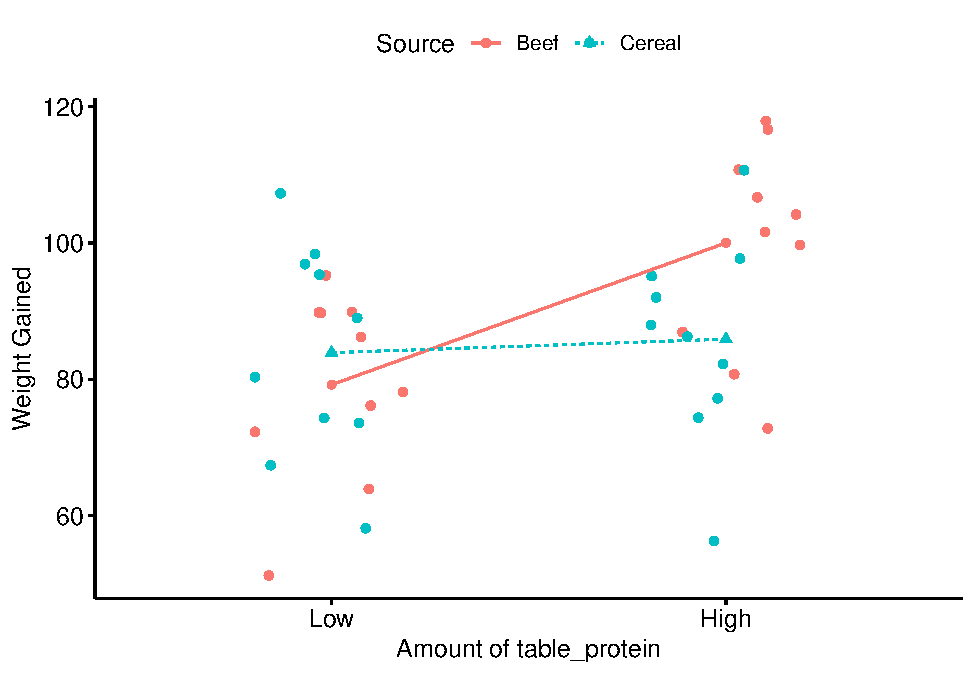
\includegraphics[width=0.3\linewidth]{lab_stat565_files/figure-latex/unnamed-chunk-3-1}

\begin{Shaded}
\begin{Highlighting}[]
\CommentTok{#Plots the Mean and 1SD error bars for each treatment group #}
\KeywordTok{ggplot}\NormalTok{(}\DataTypeTok{data =}\NormalTok{ table_protein, }\KeywordTok{aes}\NormalTok{(}\DataTypeTok{x =}\NormalTok{ Amount, }\DataTypeTok{y =}\NormalTok{ Gain, }\DataTypeTok{colour=}\NormalTok{Source,}\DataTypeTok{shape =}\NormalTok{ Source, }\DataTypeTok{group=}\NormalTok{Source)) }\OperatorTok{+}
\StringTok{  }\KeywordTok{stat_summary}\NormalTok{() }\OperatorTok{+}\StringTok{ }\KeywordTok{labs}\NormalTok{(}\DataTypeTok{y=} \StringTok{"Weight Gained"}\NormalTok{, }\DataTypeTok{x=}\StringTok{"Amount of table_protein"}\NormalTok{, }\DataTypeTok{color=}\StringTok{"Source"}\NormalTok{, }\DataTypeTok{shape=}\StringTok{"Source"}\NormalTok{)}
\end{Highlighting}
\end{Shaded}

\begin{verbatim}
## No summary function supplied, defaulting to `mean_se()
\end{verbatim}

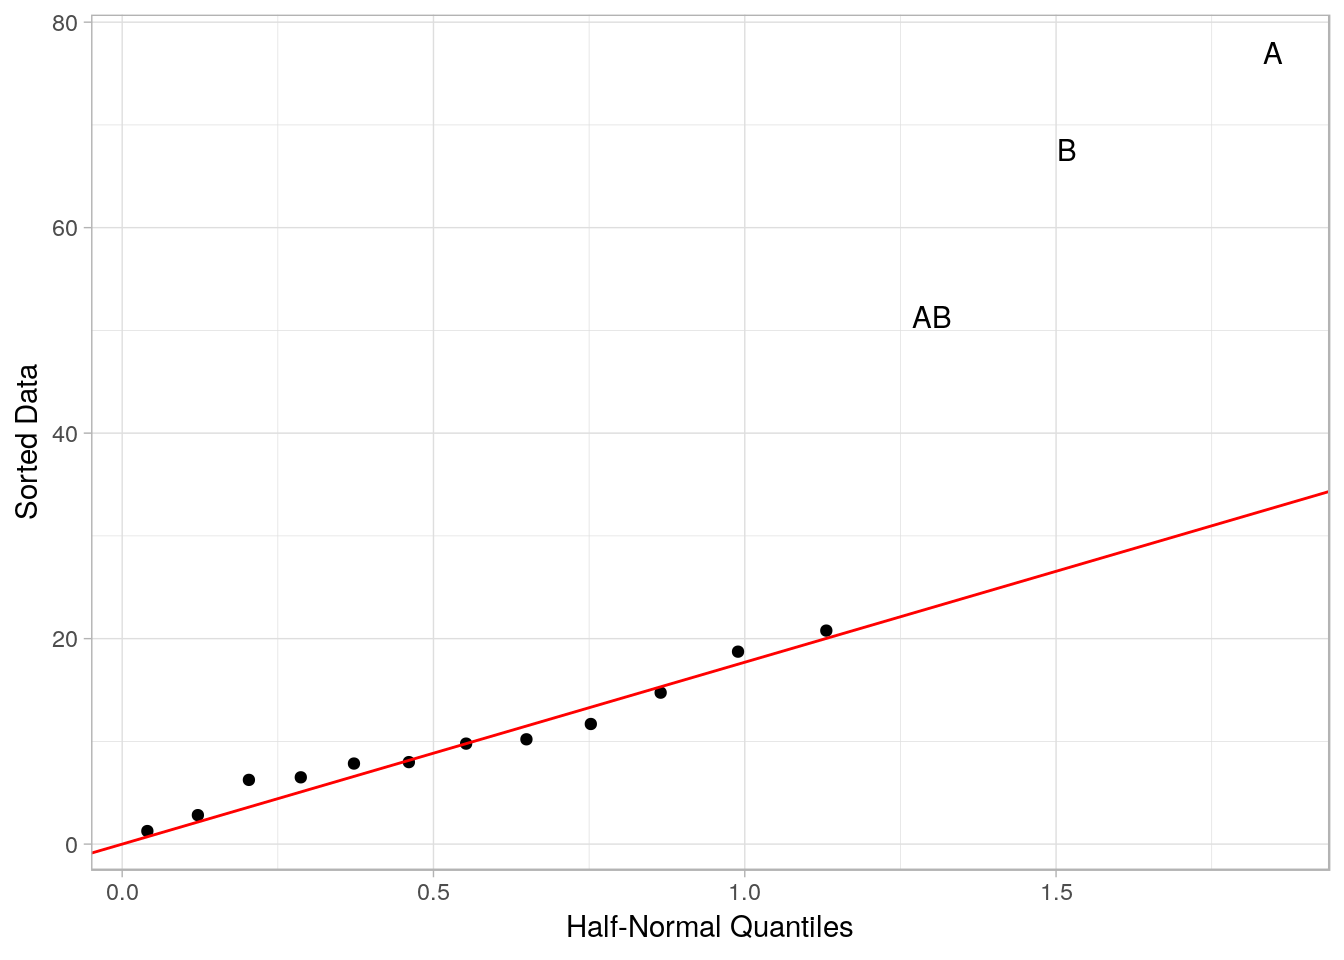
\includegraphics[width=0.3\linewidth]{lab_stat565_files/figure-latex/unnamed-chunk-3-2}

\begin{Shaded}
\begin{Highlighting}[]
\CommentTok{# Install and load ggpubr package before using ggline function # }
\KeywordTok{ggline}\NormalTok{(}\DataTypeTok{data =}\NormalTok{ table_protein, }\DataTypeTok{x =} \StringTok{"Amount"}\NormalTok{, }\DataTypeTok{y =} \StringTok{"Gain"}\NormalTok{, }\DataTypeTok{add =} \KeywordTok{c}\NormalTok{(}\StringTok{"mean"}\NormalTok{, }\StringTok{"jitter"}\NormalTok{),}\DataTypeTok{shape=} \StringTok{"Source"}\NormalTok{,  }\DataTypeTok{color =} \StringTok{"Source"}\NormalTok{, }\DataTypeTok{linetype =} \StringTok{"Source"}\NormalTok{, }\DataTypeTok{ylab=} \StringTok{"Weight Gained"}\NormalTok{, }\DataTypeTok{xlab=}\StringTok{"Amount of table_protein"}\NormalTok{)}
\end{Highlighting}
\end{Shaded}

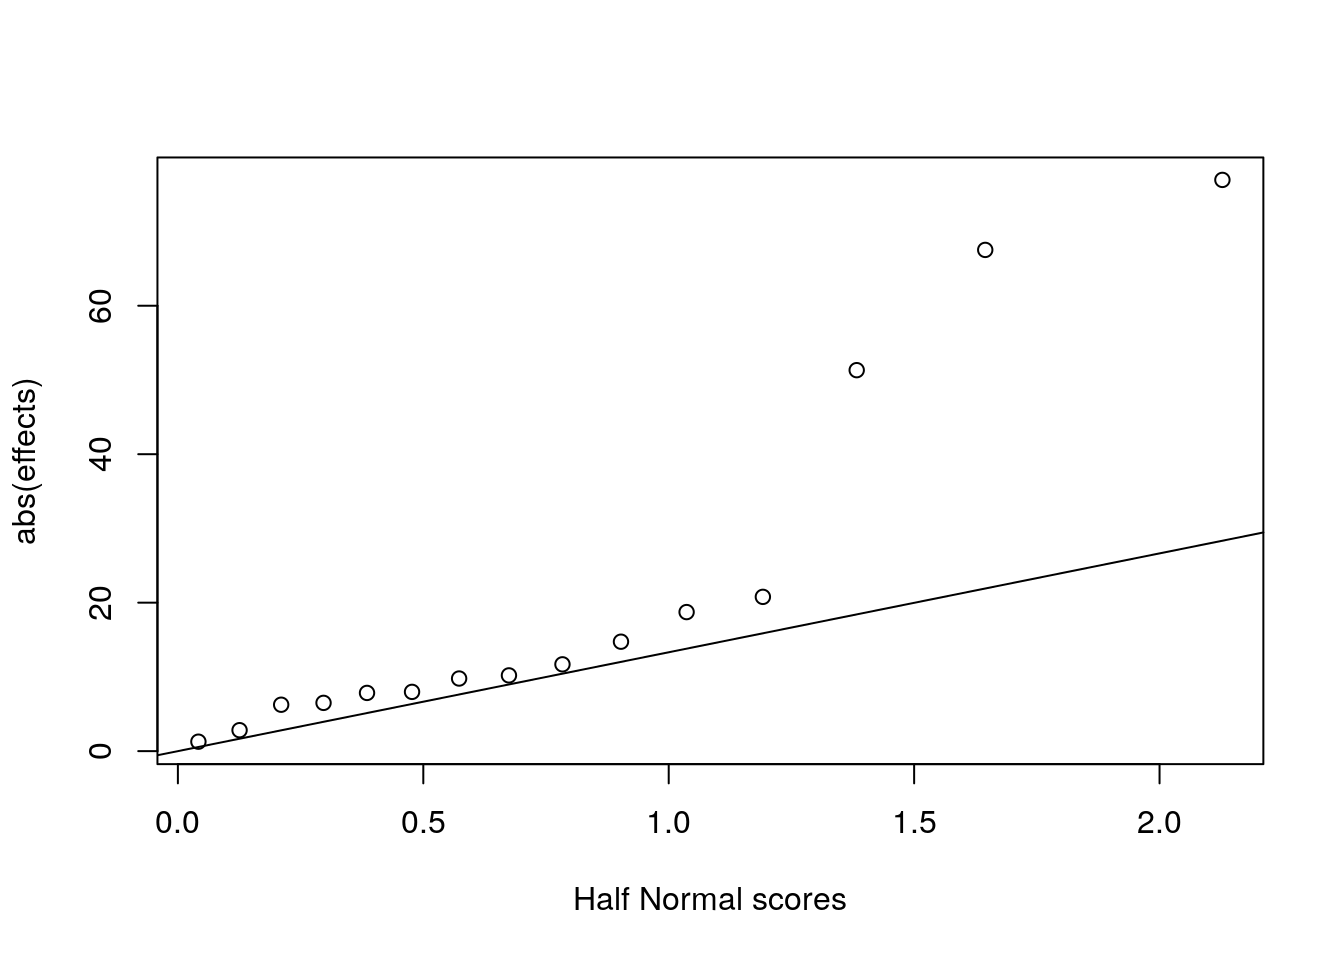
\includegraphics[width=0.3\linewidth]{lab_stat565_files/figure-latex/unnamed-chunk-3-3}

\begin{Shaded}
\begin{Highlighting}[]
\CommentTok{#Load mosaic package before using favstats function#}
\KeywordTok{favstats}\NormalTok{(Gain }\OperatorTok{~}\StringTok{ }\NormalTok{Source, }\DataTypeTok{data=}\NormalTok{table_protein)}
\end{Highlighting}
\end{Shaded}

\begin{verbatim}
##   Source min   Q1 median    Q3 max mean       sd  n missing
## 1   Beef  51 77.5     90 102.5 118 89.6 17.71232 20       0
## 2 Cereal  56 74.0     87  95.5 111 84.9 14.99438 20       0
\end{verbatim}

\begin{Shaded}
\begin{Highlighting}[]
\KeywordTok{favstats}\NormalTok{(Gain }\OperatorTok{~}\StringTok{ }\NormalTok{Amount , }\DataTypeTok{data=}\NormalTok{table_protein)}
\end{Highlighting}
\end{Shaded}

\begin{verbatim}
##   Amount min    Q1 median     Q3 max  mean       sd  n missing
## 1   High  56 81.75   93.5 104.75 118 92.95 16.36259 20       0
## 2    Low  51 73.50   83.0  91.25 107 81.55 14.63045 20       0
\end{verbatim}

\begin{Shaded}
\begin{Highlighting}[]
\KeywordTok{favstats}\NormalTok{(Gain }\OperatorTok{~}\StringTok{ }\NormalTok{Source}\OperatorTok{|}\NormalTok{Amount, }\DataTypeTok{data=}\NormalTok{table_protein)}
\end{Highlighting}
\end{Shaded}

\begin{verbatim}
##        Amount min    Q1 median     Q3 max   mean       sd  n missing
## 1   Beef.High  73 90.25  103.0 110.00 118 100.00 15.13642 10       0
## 2 Cereal.High  56 78.25   87.0  94.25 111  85.90 15.02184 10       0
## 3    Beef.Low  51 73.00   82.0  90.00  95  79.20 13.88684 10       0
## 4  Cereal.Low  58 74.00   84.5  96.50 107  83.90 15.70881 10       0
## 5        High  56 81.75   93.5 104.75 118  92.95 16.36259 20       0
## 6         Low  51 73.50   83.0  91.25 107  81.55 14.63045 20       0
\end{verbatim}

\begin{Shaded}
\begin{Highlighting}[]
\CommentTok{#favstats(Gain ~ Source+Amount, data=table_protein)}

\CommentTok{#Create Categorical variables so that plot of residuals versus each treatment combination can be obtained using plot function with the fitted model later #}
\NormalTok{table_protein}\OperatorTok{$}\NormalTok{Trt1 =}\StringTok{ }\KeywordTok{as.factor}\NormalTok{(table_protein}\OperatorTok{$}\NormalTok{Source)}
\NormalTok{table_protein}\OperatorTok{$}\NormalTok{Trt2 =}\StringTok{ }\KeywordTok{as.factor}\NormalTok{(table_protein}\OperatorTok{$}\NormalTok{Amount)}

\NormalTok{model_protein <-}\StringTok{ }\KeywordTok{aov}\NormalTok{(Gain }\OperatorTok{~}\StringTok{ }\NormalTok{Trt1}\OperatorTok{*}\NormalTok{Trt2, }\DataTypeTok{data=}\NormalTok{table_protein)}
\KeywordTok{summary}\NormalTok{(model_protein)}
\end{Highlighting}
\end{Shaded}

\begin{verbatim}
##             Df Sum Sq Mean Sq F value Pr(>F)  
## Trt1         1    221   220.9   0.988 0.3269  
## Trt2         1   1300  1299.6   5.812 0.0211 *
## Trt1:Trt2    1    884   883.6   3.952 0.0545 .
## Residuals   36   8049   223.6                 
## ---
## Signif. codes:  0 '***' 0.001 '**' 0.01 '*' 0.05 '.' 0.1 ' ' 1
\end{verbatim}

\begin{Shaded}
\begin{Highlighting}[]
\KeywordTok{plot}\NormalTok{(model_protein, }\DataTypeTok{pch=}\DecValTok{16}\NormalTok{)}
\end{Highlighting}
\end{Shaded}

\includegraphics[width=0.3\linewidth]{lab_stat565_files/figure-latex/unnamed-chunk-3-4}
\includegraphics[width=0.3\linewidth]{lab_stat565_files/figure-latex/unnamed-chunk-3-5}
\includegraphics[width=0.3\linewidth]{lab_stat565_files/figure-latex/unnamed-chunk-3-6}
\includegraphics[width=0.3\linewidth]{lab_stat565_files/figure-latex/unnamed-chunk-3-7}

\begin{Shaded}
\begin{Highlighting}[]
\CommentTok{# Pairwise comparisons using t tests with pooled Standard Deviation #}
\CommentTok{# The output gives a matrix of p values for each pair of treatments #}
\KeywordTok{pairwise.t.test}\NormalTok{(table_protein}\OperatorTok{$}\NormalTok{Gain, table_protein}\OperatorTok{$}\NormalTok{Trt2, }\DataTypeTok{p.adj =} \StringTok{"none"}\NormalTok{) }
\end{Highlighting}
\end{Shaded}

\begin{verbatim}
## 
##  Pairwise comparisons using t tests with pooled SD 
## 
## data:  table_protein$Gain and table_protein$Trt2 
## 
##     High 
## Low 0.026
## 
## P value adjustment method: none
\end{verbatim}

\begin{Shaded}
\begin{Highlighting}[]
\CommentTok{# Pairwise comparisons using t tests with pooled Standard Deviation and Bonferroni adjustment #}
\CommentTok{# The output gives a matrix of p values for each pair of treatments #}
\KeywordTok{pairwise.t.test}\NormalTok{(table_protein}\OperatorTok{$}\NormalTok{Gain, table_protein}\OperatorTok{$}\NormalTok{Trt2, }\DataTypeTok{p.adj =} \StringTok{"bonf"}\NormalTok{)}
\end{Highlighting}
\end{Shaded}

\begin{verbatim}
## 
##  Pairwise comparisons using t tests with pooled SD 
## 
## data:  table_protein$Gain and table_protein$Trt2 
## 
##     High 
## Low 0.026
## 
## P value adjustment method: bonferroni
\end{verbatim}

\begin{Shaded}
\begin{Highlighting}[]
\CommentTok{#Install and load the agricolae package before running the LSD.test function below #}
\CommentTok{#p.adj option in the LSD.test function can be used to apply different adjustments to control error rates#}
\KeywordTok{plot}\NormalTok{(}\KeywordTok{LSD.test}\NormalTok{(model_protein, }\DataTypeTok{trt =} \StringTok{"Trt2"}\NormalTok{, }\DataTypeTok{alpha =} \FloatTok{0.05}\NormalTok{))}
\end{Highlighting}
\end{Shaded}

\includegraphics[width=0.3\linewidth]{lab_stat565_files/figure-latex/unnamed-chunk-3-8}

\begin{Shaded}
\begin{Highlighting}[]
\CommentTok{#The treatments sharing the same letter on the plot are not different#}

\NormalTok{(}\KeywordTok{LSD.test}\NormalTok{(model_protein, }\DataTypeTok{trt =} \StringTok{"Trt2"}\NormalTok{, }\DataTypeTok{alpha =} \FloatTok{0.05}\NormalTok{)) }\CommentTok{# Using outer parentheses prints the output#}
\end{Highlighting}
\end{Shaded}

\begin{verbatim}
## $statistics
##    MSerror Df  Mean       CV  t.value  LSD
##   223.5944 36 87.25 17.13819 2.028094 9.59
## 
## $parameters
##         test p.ajusted name.t ntr alpha
##   Fisher-LSD      none   Trt2   2  0.05
## 
## $means
##       Gain      std  r      LCL      UCL Min Max   Q25  Q50    Q75
## High 92.95 16.36259 20 86.16885 99.73115  56 118 81.75 93.5 104.75
## Low  81.55 14.63045 20 74.76885 88.33115  51 107 73.50 83.0  91.25
## 
## $comparison
## NULL
## 
## $groups
##       Gain groups
## High 92.95      a
## Low  81.55      b
## 
## attr(,"class")
## [1] "group"
\end{verbatim}

\begin{Shaded}
\begin{Highlighting}[]
\CommentTok{#Tukey's test to get observed difference in means, CI and p value#}
\KeywordTok{TukeyHSD}\NormalTok{(model_protein, }\DataTypeTok{conf.level =} \FloatTok{0.95}\NormalTok{)}
\end{Highlighting}
\end{Shaded}

\begin{verbatim}
##   Tukey multiple comparisons of means
##     95% family-wise confidence level
## 
## Fit: aov(formula = Gain ~ Trt1 * Trt2, data = table_protein)
## 
## $Trt1
##             diff    lwr  upr     p adj
## Cereal-Beef -4.7 -14.29 4.89 0.3268783
## 
## $Trt2
##           diff    lwr   upr     p adj
## Low-High -11.4 -20.99 -1.81 0.0211449
## 
## $`Trt1:Trt2`
##                         diff      lwr       upr     p adj
## Cereal:High-Beef:High  -14.1 -32.1102  3.910198 0.1697711
## Beef:Low-Beef:High     -20.8 -38.8102 -2.789802 0.0182745
## Cereal:Low-Beef:High   -16.1 -34.1102  1.910198 0.0936982
## Beef:Low-Cereal:High    -6.7 -24.7102 11.310198 0.7492577
## Cereal:Low-Cereal:High  -2.0 -20.0102 16.010198 0.9905411
## Cereal:Low-Beef:Low      4.7 -13.3102 22.710198 0.8952934
\end{verbatim}

\begin{Shaded}
\begin{Highlighting}[]
\CommentTok{# Scheffe's test to get observed difference in means, CI and p value #}
\CommentTok{# Install and load the DescTools package before using the ScheffeTest function #}
\KeywordTok{ScheffeTest}\NormalTok{(model_protein, }\DataTypeTok{conf.level =} \FloatTok{0.95}\NormalTok{)}
\end{Highlighting}
\end{Shaded}

\begin{verbatim}
## 
##   Posthoc multiple comparisons of means : Scheffe Test 
##     95% family-wise confidence level
## 
## $Trt1
##             diff    lwr.ci   upr.ci   pval    
## Cereal-Beef -4.7 -18.56594 9.165941 0.8042    
## 
## $Trt2
##           diff    lwr.ci   upr.ci   pval    
## Low-High -11.4 -25.26594 2.465941 0.1410    
## 
## $`Trt1:Trt2`
##                         diff   lwr.ci    upr.ci   pval    
## Cereal:High-Beef:High  -14.1 -33.7094  5.509402 0.2358    
## Beef:Low-Beef:High     -20.8 -40.4094 -1.190598 0.0338 *  
## Cereal:Low-Beef:High   -16.1 -35.7094  3.509402 0.1418    
## Beef:Low-Cereal:High    -6.7 -26.3094 12.909402 0.8004    
## Cereal:Low-Cereal:High  -2.0 -21.6094 17.609402 0.9929    
## Cereal:Low-Beef:Low      4.7 -14.9094 24.309402 0.9195    
## 
## ---
## Signif. codes:  0 '***' 0.001 '**' 0.01 '*' 0.05 '.' 0.1 ' ' 1
\end{verbatim}


\end{document}
